% !TEX root = ../agglo_clust_review.tex

\section{Introduction}
%On possible selling story could be: currently many of the successful proposal-free instance segmentation methods rely on a final clustering step on a grid-graph with both short and long-range connections. So it is worth to study this problem in more details. 

Deep convolutional neural nets (CNNs) has been successfully applied to a wide range of tasks of computer vision and pixel-level image understanding, such as \UPDATE{boundary detection \cite{arbelaez2011contour,xie2015holistically,maninis2018convolutional}, semantic segmentation \cite{long2015fully,chen2018deeplab,kong2018recurrent}, optical flow \cite{weinzaepfel2013deepflow,dosovitskiy2015flownet}, and pose estimation \cite{wei2016convolutional,cao2017realtime}.}


\begin{itemize}
% \SOURCE{\cite{kong2018recurrent}}
\item \emph{Instance segmentation} is a task of computer vision that involves the detection of all objects in an image by performing pixel-level segmentation of each instance.   
\item Many recent successful methods for instance segmentation %, usually named \emph{proposal-based methods}, 
 use heuristic approaches that start from the classical computer vision task of \emph{object detection}, where the goal is to localize each objects using a bounding box, and then predict both a pixel-level mask of each instance and a semantic label (classify the objects in the bounding box). \TODO{Is it really general enough as a description...?} \cite{yang2012layered,ladicky2010and,hariharan2014simultaneous,chen2015multi,dai2016instance,liang2016reversible,he2017mask}
\item While effective, these approaches are \UPDATE{somewhat unsatisfying (copy/paste, change: present some faults)} because:
\begin{itemize}
\item they rely on the object detector and non-maximum suppression heuristics to count how many instances are present in the image, 
\item they tend to underperform in cluttered scenes, since instance assignment is often carried out independently for each detection; 
\item they are not usable for wiry or articulated objects (e.g. in the field of connectomics and neuron segmenation from electron microscopy images) 
\item their architecture do not usually prevent a pixel to be shared between multiple instances
\item they do not scale up well since each proposal has to be singularly processed by the CNN. 
% \item (difficult to train in an end-to-end manner: interface between instance segmentation and detection is non-differentiable)
% \item (architecture is complex and hard to tune and “debug”...?)
\end{itemize}

\item Currently there are two successful approaches used for proposal-free instance segmentation: the first ones predict associative pixel embedding vectors, where the goal is to have a CNN predicting embedding vectors that are similar only for pixels in the same instance \cite{kong2018recurrent,fathi2017semantic,newell2017associative,de2017semantic}; in the second type of approaches, for every pixel a set of neighboring pixels is fixed  (not necesarelly limited to the direct neighbors) and a CNN then predicts affinities, that represent how likelity it is for each of neighboring pixels to be in the same instance \cite{liu2018affinity,wolf2018mutex,xie2015holistically}

\item Both approaches requires a final clustering algorithm to output the final instance segmentation 

 and we can define a grid graph, where each vertex represents a pixel, with short- and long-range edge connections 

 and find the final instance segmentation by using a graph clustering algorithm.

\item Recent work (\cite{wolf2018mutex}, more...) shows that it is better to use \textbf{repulsion and attraction} (directly predict it with the classifier, no need to define seeds or to fix a threshold given an hierarchy of clusters)
\item solving correlation clustering problem (multicut) is too expensive for this application (even using recently proposed heuristics)
\item our contributions:
\begin{itemize}
\item we propose a unified and simple formalization of Agglomerative Clustering and show how many of the recently proposed methods can be seen as special cases (focusing in particular on signed graphs) (\textbf{review and comparison paper})
\item new clustering algorithms on signed graphs
\item we compare different types of agglomeration clustering on a pixel grid graph with short and long-range connections, focusing on aspects like efficieny, robustness (and MC energy) 

\end{itemize}
\item on other datasets (connectomics) many methods are based on multi-step pipelines first predicting superpixels
\item \textit{if we get good scores on CREMI}: we show that also on neuro-data it is worth to skip the hand-crafted superpixel step and compute the final segmentation directly from the CNN affinities (MWS already showed it on the ISBI dataset)

\end{itemize}


\begin{figure}[t]
\centering
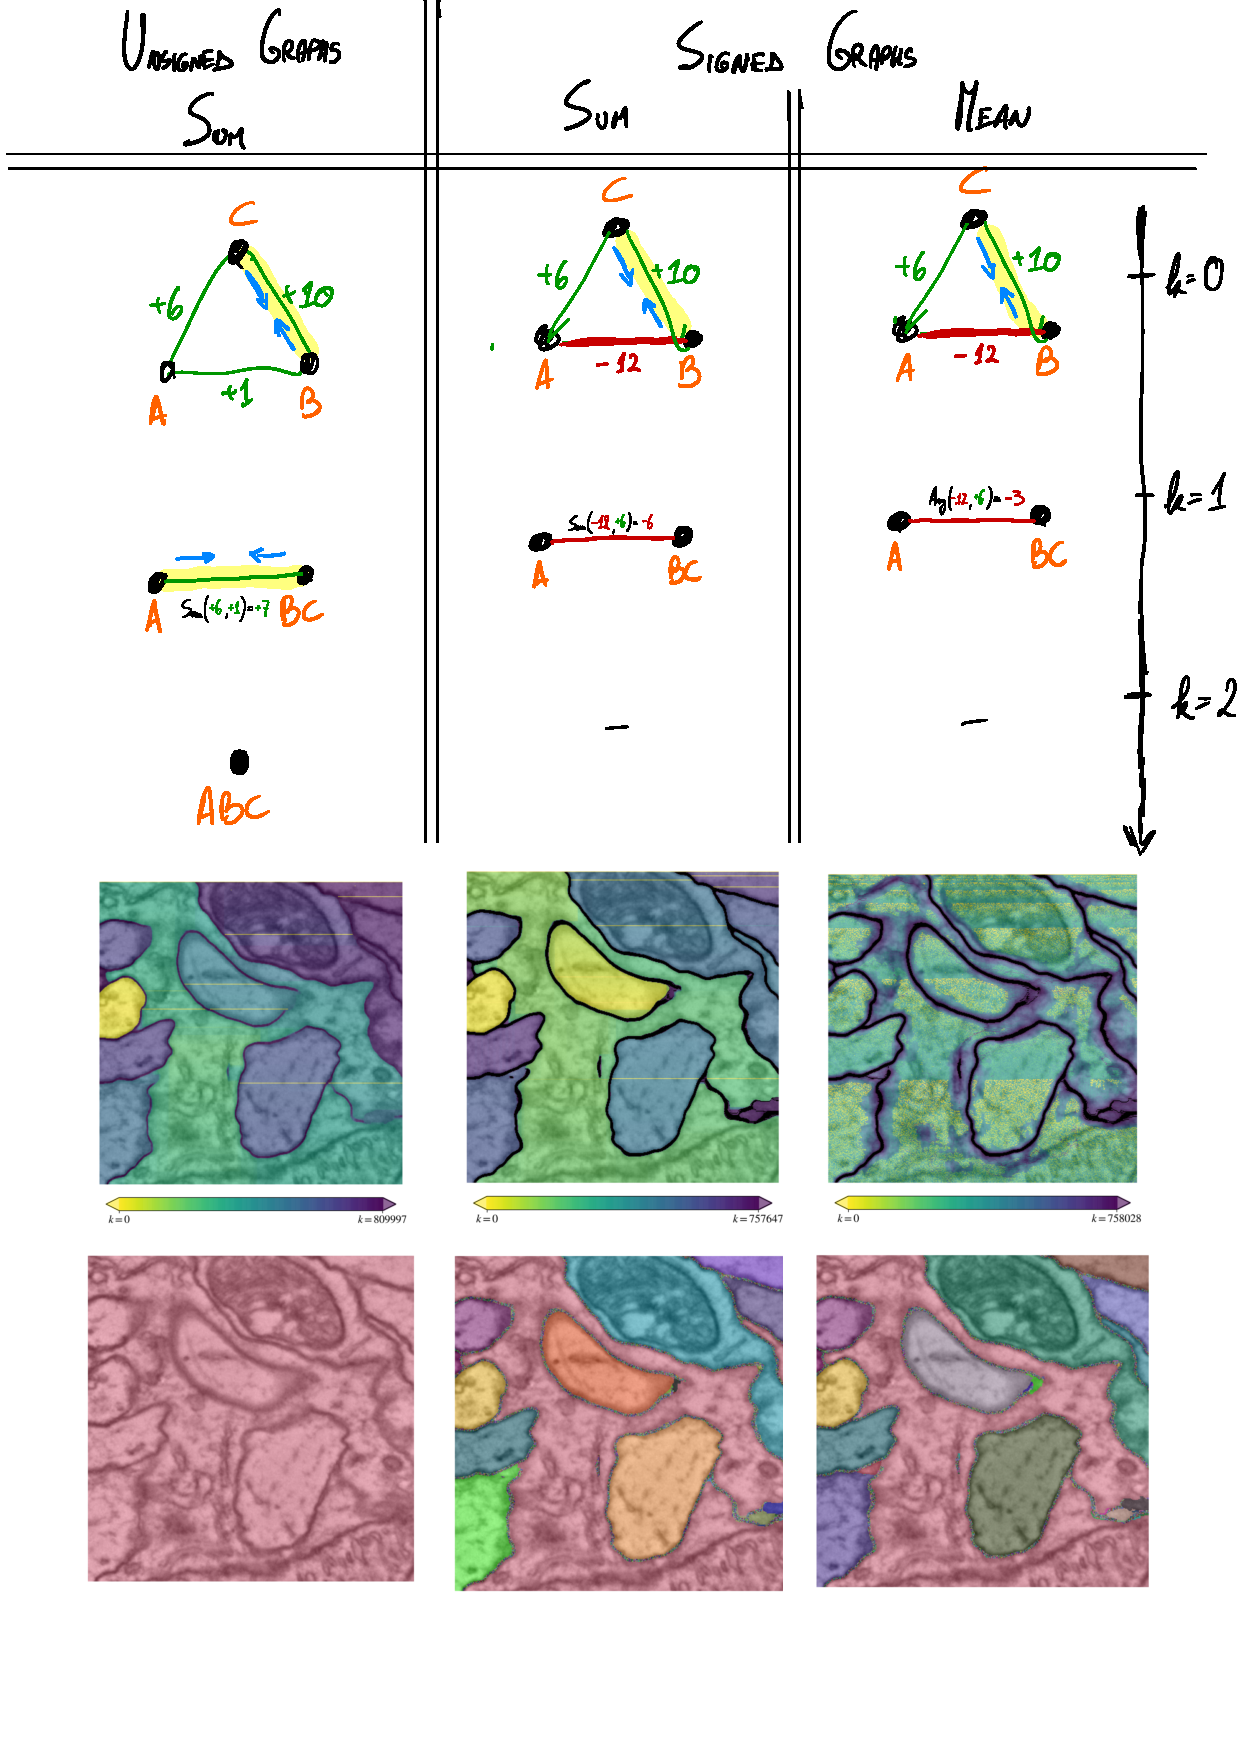
\includegraphics[width=\textwidth,trim=0.4in 1.2in 0.in 0.05in,clip]{./figs/intro_image.jpg} % left bottom right top
\caption{\small 
Intro image: explain algorithm, main ideas and contributions
\label{fig:intro_figure}}
\end{figure}
